\documentclass{article}
\usepackage{microtype,graphicx,booktabs,amsmath,amssymb,amsthm,hyperref}
\usepackage[preprint]{icml2026}
\newtheorem{theorem}{Theorem}
\newtheorem{proposition}{Proposition}
\newtheorem{corollary}{Corollary}
\newcommand{\R}{\mathbb{R}}
\newcommand{\norm}[1]{\left\|#1\right\|}
\newcommand{\ip}[2]{\langle #1,#2\rangle}
\newcommand{\A}{\mathcal{A}}
\icmltitlerunning{Auditing Density Uncertainty Beyond the Reconstruction Dictionary}
\begin{document}
\twocolumn[
\icmltitle{Auditing Density Uncertainty in Cryo-EM\\Beyond a Gaussian Reconstruction Dictionary}
\begin{icmlauthorlist}\icmlauthor{Anonymous Authors}{anon}\end{icmlauthorlist}
\icmlaffiliation{anon}{Fourier Cryo Splats research project}
\icmlcorrespondingauthor{Project repository}{\url{https://github.com/yashpatel5400/fourier-cryo-splats}}
\icmlkeywords{cryo-EM, uncertainty quantification, inverse problems, Gaussian splats}
\vskip 0.2in]
\printAffiliationsAndNotice{}
\hypersetup{pdftitle={Auditing Density Uncertainty in Cryo-EM Beyond a Gaussian Reconstruction Dictionary},pdfsubject={Development preprint in ICML format; not submitted or accepted}}
\begin{center}\small\textbf{Development manuscript, 29 September 2026.}\\
Preliminary experiments; not a completed submission candidate.
\end{center}
\begin{abstract}
A confidence interval can be calibrated within a reconstruction dictionary and still miss errors excluded by that dictionary. We investigate this failure in cryogenic electron microscopy (cryo-EM), using conjugate-paired Fourier Gaussians as a computational representation. Our candidate procedure estimates fixed linear density features and audits their bias through the adjoint residual in an explicitly larger voxel space. This separates numerical representation from the density class to which a confidence statement applies. We specialize classical bias-aware inference to the Fourier-slice model, derive explicit bounds for local pose errors, and implement reduced-space and matrix-free solvers with primal-dual diagnostics. Development experiments include repeated bounded-model tests and acquisition geometries from three experimental particle stacks. In fixed-pose tests, dictionary-only intervals can severely undercover an independent map generator; an ambient-space audit restores the assumed-model guarantee. Broader features admit useful intervals, while finer features and restricted viewing angles expose large uncertainty. Density radii, support, Gaussian noise and pose bounds remain explicit assumptions. Comprehensive end-to-end validation, several external baselines and independent review are outstanding; these preliminary results do not establish publication readiness.
\end{abstract}

\section{Introduction}
Cryo-EM reconstructs molecular density from noisy projections whose orientations, translations and imaging parameters are imperfectly known. Modern neural and Gaussian representations offer expressive reconstruction models, but expressiveness alone does not establish which reconstructed features the data support. We focus on a fixed local density average or contrast. This target differs from a conformational population, the uncertainty of an atomic model, or prediction of a noisy held-out particle image.

An uncertainty calculation usually inherits its reconstruction space. If a Gaussian dictionary spans $S$, a posterior or confidence interval computed in $S$ need not cover density outside $S$. Improving optimization inside the dictionary does not remove this discrepancy. Independent half reconstructions can also share the same representational restriction. Our working question is whether one can retain Gaussian computation while auditing feature uncertainty in a larger, explicitly declared density class.

We develop three connected components: an adjoint-residual audit that separates fitting and inference spaces; a Fourier-Gaussian treatment of bounded local pose errors, including the density--pose interaction and a uniform nonlinear remainder; and a validation protocol that distinguishes fixed-parameter coverage, Bayesian prior-predictive coverage and experimental-image prediction. We do not claim a new general theory of bias-aware intervals, reduced-space duality or primal-dual optimization. The value of the cryo-EM specialization must be established by its usefulness, assumptions and comparison to existing methods.

\section{Related Work and Scientific Scope}
\paragraph{Probabilistic reconstruction.} Bayesian inference is foundational in cryo-EM \citep{scheres2012}. \citet{ullrich2020} already combine differentiable Fourier-slice reconstruction with variational density uncertainty and discuss the distinction between variance and model bias. \citet{rangan2024} examine soft modes of the joint volume/alignment likelihood Hessian. Thus neither a probabilistic Fourier representation nor pose--density ambiguity is a new observation. Our candidate emphasizes a finite-sample, bounded-class statement and a check outside the fitting dictionary.

\paragraph{Representations and heterogeneity.} CryoDRGN learns a latent-conditioned density family \citep{zhong2021}; its latent variation is not automatically calibrated uncertainty in a homogeneous density. Ab initio neural inference \citep{zhong2021b} is a different task from fixed-pose backprojection. Gaussian mixtures and Gaussian splatting are also established \citep{chen2021,chen2025,qu2025,shekar2025}. We use Fourier kernels as a numerical basis, without treating their existence as the contribution. Continuous-state recovery, conformational populations and pose entanglement are substantial separate problems; the living survey records current RECOVAR, DynaMight, cryoDRGN-AI and CAHRA work with source-level distinctions.

\paragraph{Validation and map confidence.} Gold-standard splitting and noise substitution address reconstruction overfitting \citep{schereschen2012,chen2013}; a shell correlation is not a coverage statement for a local feature. LocScale-2.0 provides calibrated confidence for map enhancement relative to its reference target \citep{locscale2026}. That target must not be conflated with confidence in an unknown density from raw particles. Map significance relative to background noise, directional resolution, atomic-model reliability and particle-derived confidence likewise answer different questions.

\paragraph{Statistical foundations.} Optimal recovery links linear inverse estimation to bias--variance tradeoffs \citep{donoho1994}. Honest inference over convex function classes and bias-aware Gaussian critical values are classical \citep{armstrong2018}. Our theorems below specialize these principles and identify the assumptions that cryo-EM introduces. The survey and its bibliographic ledger are ongoing; a downloaded paper is not counted as a completed critical review.

\section{Forward Model and Inference Target}
With $F(k)=\int\rho(x)e^{-2\pi i k^\top x}\,dx$, a particle obeys
\begin{equation}
Y_i(q)=C_i(q)e^{-2\pi i q^\top t_i}F(E_iq)+\epsilon_i(q).
\end{equation}
$E_i$ embeds a detector plane, $C_i$ is its contrast transfer function (CTF), and frequencies and translations use reciprocal units. We realify one representative of each conjugate Fourier pair and whiten the noise. The initial theory conditions on a fixed design and an independent pilot $\rho_0$, giving
\begin{equation}\label{eq:model}
y-\A\rho_0=\A\delta+Ju+r+\epsilon,\quad\epsilon\sim N(0,I).
\end{equation}
Here $\delta=\rho-\rho_0$, $J$ is block diagonal over particles, $u$ describes bounded nuisance errors, and $r$ is a bounded remainder. We assume
\begin{equation}\label{eq:class}
\norm{\delta}_{H}\le B,\quad\norm{u_i}\le\eta_i,\quad\norm{r_i}\le\gamma_i.
\end{equation}
$H$ is either a declared Gaussian density subspace or an ambient voxel space with a stated support mask. These are different classes. A physical density-energy norm includes voxel volume; experiments using an ordinary voxel Euclidean norm explicitly normalize that norm. $B$, $\eta_i$ and $\gamma_i$ are assumptions, not quantities automatically learned from residual fit.

The estimand is $t=\ip{\ell}{\rho}$, such as a Gaussian-weighted spatial average or the difference of two such averages. The smoothing scale and coordinate frame are specified in physical units. For weights fixed without the inference noise, use
\begin{equation}\label{eq:estimator}
\widehat t=\ip{\ell}{\rho_0}+w^\top(y-\A\rho_0).
\end{equation}
The pilot, dictionary, whitening, target and weights may depend on independent development data. Poses estimated from the inference images violate literal fixed-design independence; supplied consensus poses therefore support only a conditional experimental analysis here.

\section{Bias-Aware Confidence and Ambient Auditing}
\subsection{A conditional certificate}
Define $s=\norm{w}$ and
\begin{align}\label{eq:bias}
b_H(w)&=B\norm{\ell-\A^*w}_{H}\nonumber\\
&\quad+\sum_i\eta_i\norm{J_i^\top w_i}+\sum_i\gamma_i\norm{w_i}.
\end{align}
Let $q(s,b,\alpha)$ solve
\begin{equation}\label{eq:critical}
\Phi((q-b)/s)-\Phi((-q-b)/s)=1-\alpha
\end{equation}
when $s>0$, and set $q(0,b,\alpha)=b$.
\begin{theorem}[Conditional coverage]\label{thm:coverage}
Under Equations~\eqref{eq:model}--\eqref{eq:class}, the interval
$\widehat t\pm q(s,b_H(w),\alpha)$ covers $t$ with probability at least $1-\alpha$, uniformly over the stated class, conditional on the independent design choices.
\end{theorem}
\begin{proof}
The deterministic estimation error is
$\ip{\A^*w-\ell}{\delta}+\sum_iw_i^\top J_i u_i+\sum_iw_i^\top r_i$.
Cauchy--Schwarz bounds its absolute value by $b_H$. The remaining error is Gaussian with standard deviation $s$. Coverage of a symmetric interval decreases with the absolute Gaussian mean, so the minimum occurs at mean $\pm b_H$ and equals Equation~\eqref{eq:critical}.
\end{proof}
The result is a direct bias-aware inference construction. It is useful only if its assumptions are defensible and its width improves on the no-data interval $\ip{\ell}{\rho_0}\pm B\norm{\ell}$.

\subsection{Why auditing the dictionary matters}
Let $S:\R^p\to H$ have orthonormal columns. A restricted calculation replaces the density term by $B\norm{S^*(\ell-\A^*w)}$. Write $h=\ell-\A^*w$. Then
\begin{equation}\label{eq:orthogonal}
\norm{h}_H^2=\norm{S^*h}^2+\norm{(I-SS^*)h}_H^2.
\end{equation}
The second term measures uncertainty discarded by the dictionary. It can be large even when the restricted residual is zero. Evaluating the full adjoint residual repairs this omission for $H$ without estimating a representation-error direction from noisy data. It does not cover density outside the declared ambient grid or support.

Centering in Equation~\eqref{eq:estimator} also uses the ambient operator. If a surrogate centers the images instead, the discrepancy $w^\top(\A-\widetilde\A)\rho_0$ requires an additional bound. We do not silently substitute a surrogate forward model into the coverage theorem.

\subsection{Optimization and verifiable stopping}
We optimize the conservative convex objective
\begin{equation}\label{eq:objective}
\mathcal F_H(w)=z_{1-\alpha/2}\norm{w}+b_H(w),
\end{equation}
then report the sharper width from Equation~\eqref{eq:critical}. Its dual is
\begin{align}
\max_{v,a,d}\quad&\ip{\ell}{v}\nonumber\\
\text{s.t.}\quad&\norm{v}\le B,\ \norm{a_i}\le\eta_i,\ \norm{d_i}\le\gamma_i,\nonumber\\
&\norm{\A v-Ja-d}\le z_{1-\alpha/2}.\label{eq:dual}
\end{align}
Representing each norm by a Euclidean support function proves this dual; continuity and coercivity yield strong duality. A feasible dual iterate supplies a lower bound before convergence. The gap concerns Equation~\eqref{eq:objective}, not optimality of the folded-normal width.

For a reduced density space $S$, a feasible dual vector lifts to $Sv$ in $H$. Thus a restricted dual lower bound and an ambient primal upper bound bracket the same full-space optimum. We enrich $S$ with the component of $\ell-\A^*w$ orthogonal to it, using only design and target information. Restricted exact optima increase under enrichment; individual ambient primal values need not decrease, so we keep the best feasible iterate. No convergence-rate claim is made for this greedy construction.

Quadratic majorization gives coefficient-space conjugate-gradient solves with particle-block inverses. A classical Chambolle--Pock implementation is an alternative \citep{chambolle2011}. For fixed poses, a full-space matrix-free comparator solves $(\A^*\A+\lambda I)v=\ell$ within majorization. It can outperform enrichment and is included to prevent an unsupported Gaussian speed claim.

\section{Fourier Gaussians and Local Pose Errors}
We use smooth conjugate pairs
\begin{align}
F_c(k)&=\sum_j c_jg_j(k)+\overline c_jg_j(-k),\nonumber\\
 g_j(k)&=e^{-\norm{k-\mu_j}^2/(2\sigma_j^2)}.
\end{align}
This enforces Hermitian symmetry. Hard cutoff kernels from the earlier reconstruction prototype are unsuitable for an unqualified Taylor bound; the uncertainty implementation uses full Gaussians. Their analytic whole-space Gram matrix provides density-energy coordinates $\delta=T\beta$ with $T^*GT=I$, so $\norm{\beta}\le B$ is a density-energy assumption rather than an arbitrary coefficient scale.

Parameterize local rotations by a Lie-algebra vector and translations by detector shifts. Normalize their joint vector so $\norm{u_i}\le1$, with physical radii incorporated in the operator. With $D_{ia}=\partial A_i/\partial u_{ia}$ at the pilot pose,
\begin{align}
A_i(u_i)(c_0+\delta)&=A_i(0)(c_0+\delta)+J_i u_i\nonumber\\
&\quad+\sum_a u_{ia}D_{ia}\delta+e_i.\label{eq:pose}
\end{align}
If $H_i$ uniformly bounds the pilot's second derivative along all allowed segments and $K_i$ bounds the corresponding operator derivative, then $\norm{e_i}\le(H_i+BK_i)/2$. Define $T_i(w_i)=[D_{i1}^\top w_i,\ldots,D_{iq}^\top w_i]$. The interaction contributes at most
\begin{equation}
B\sum_i\norm{T_i(w_i)}_{\rm op}\le B\sum_i\norm{T_i(w_i)}_{F}.
\end{equation}
The implemented Frobenius relaxation is a sum of Euclidean group norms. It ignores some sharing of $\delta$ across particles and can be conservative. Charging the entire first-order interaction to an isotropic remainder was substantially worse in development.

The same construction operates in the full supported voxel space. For voxel position $x$, box length $d$, rotation radius $a$ and shift radius $s_t$, set
\begin{align}
L(q,x)&=\tfrac{2\pi}{d}(a\norm{k}\norm{x}+s_t\norm{q}),\\
H(q,x)&=\tfrac{2\pi}{d}a^2\norm{k}\norm{x}.
\end{align}
The absolute second derivative of its complex Fourier column is bounded uniformly by $|C_i(q)|[L(q,x)^2+H(q,x)]$ before whitening. Summing this column bound against $|\rho_0(x)|$ gives the pilot bound; its frequency/voxel Frobenius norm gives the operator bound. Analytic first derivatives supply the full-density interaction. Thus the implemented joint certificate covers the stated ambient density ball and local pose balls simultaneously. Fixed CTFs and known whitened Gaussian noise remain assumptions; CTF error, window correlations and heterogeneous densities are not covered by assertion.

\section{Development Experiments}
All results below are exploratory. A confirmatory protocol has not been frozen. Experimental particle pools have already been inspected during the earlier reconstruction study and subsequent development; their partitions must not be described as untouched final tests.

\subsection{Data, references and provenance}
We retain 8,192 extracted experimental images from each of EMPIAR-10028, 10049 and 10076 \citep{empiar10028,empiar10049,empiar10076}. Source exposure groups are reconstructed from deposited metadata. EMPIAR-10076 requires the original Frealign \texttt{FILM} field because its STAR micrograph numbers are sequential particle identifiers. Hash-based whole-group partitions provide pilot, tuning, inference-half and test labels within this development pool. Consensus poses and CTFs remain conditional inputs.

Deposited maps EMD-2660, EMD-6487 and EMD-8434 define independent voxel signal generators after explicit low-pass resampling. They are simulation truth, not proof of experimental accuracy. Nonuniform Fourier transforms project these maps independently of the Gaussian representation. Native and downloaded-file hashes, source indices, signs, field sizes and software versions are recorded.

\subsection{Representation and exact-dictionary controls}
A noiseless projection audit with 256 particles per split and a radius-six frequency band found relative held-out errors of approximately 1.8\%, 2.7\% and 7.7\% for the finest tested Gaussian dictionary. These residuals demonstrate why noise-only intervals do not cover representation error.

The bounded-model coverage benchmark has 48 settings: 12 seeds, broad versus preferred orientations, and rotation radii $0.5^\circ$ or $2^\circ$. Each setting uses 96 particles, 40 coefficients, 20 random bounded signals and estimator-specific adversarial controls. We report exact Gaussian noise-marginal coverage and cross-check with 2,000 paired noise draws per signal. Shared designs and paired noise do not constitute independent voxel trials.

\begin{figure*}[t]
\centering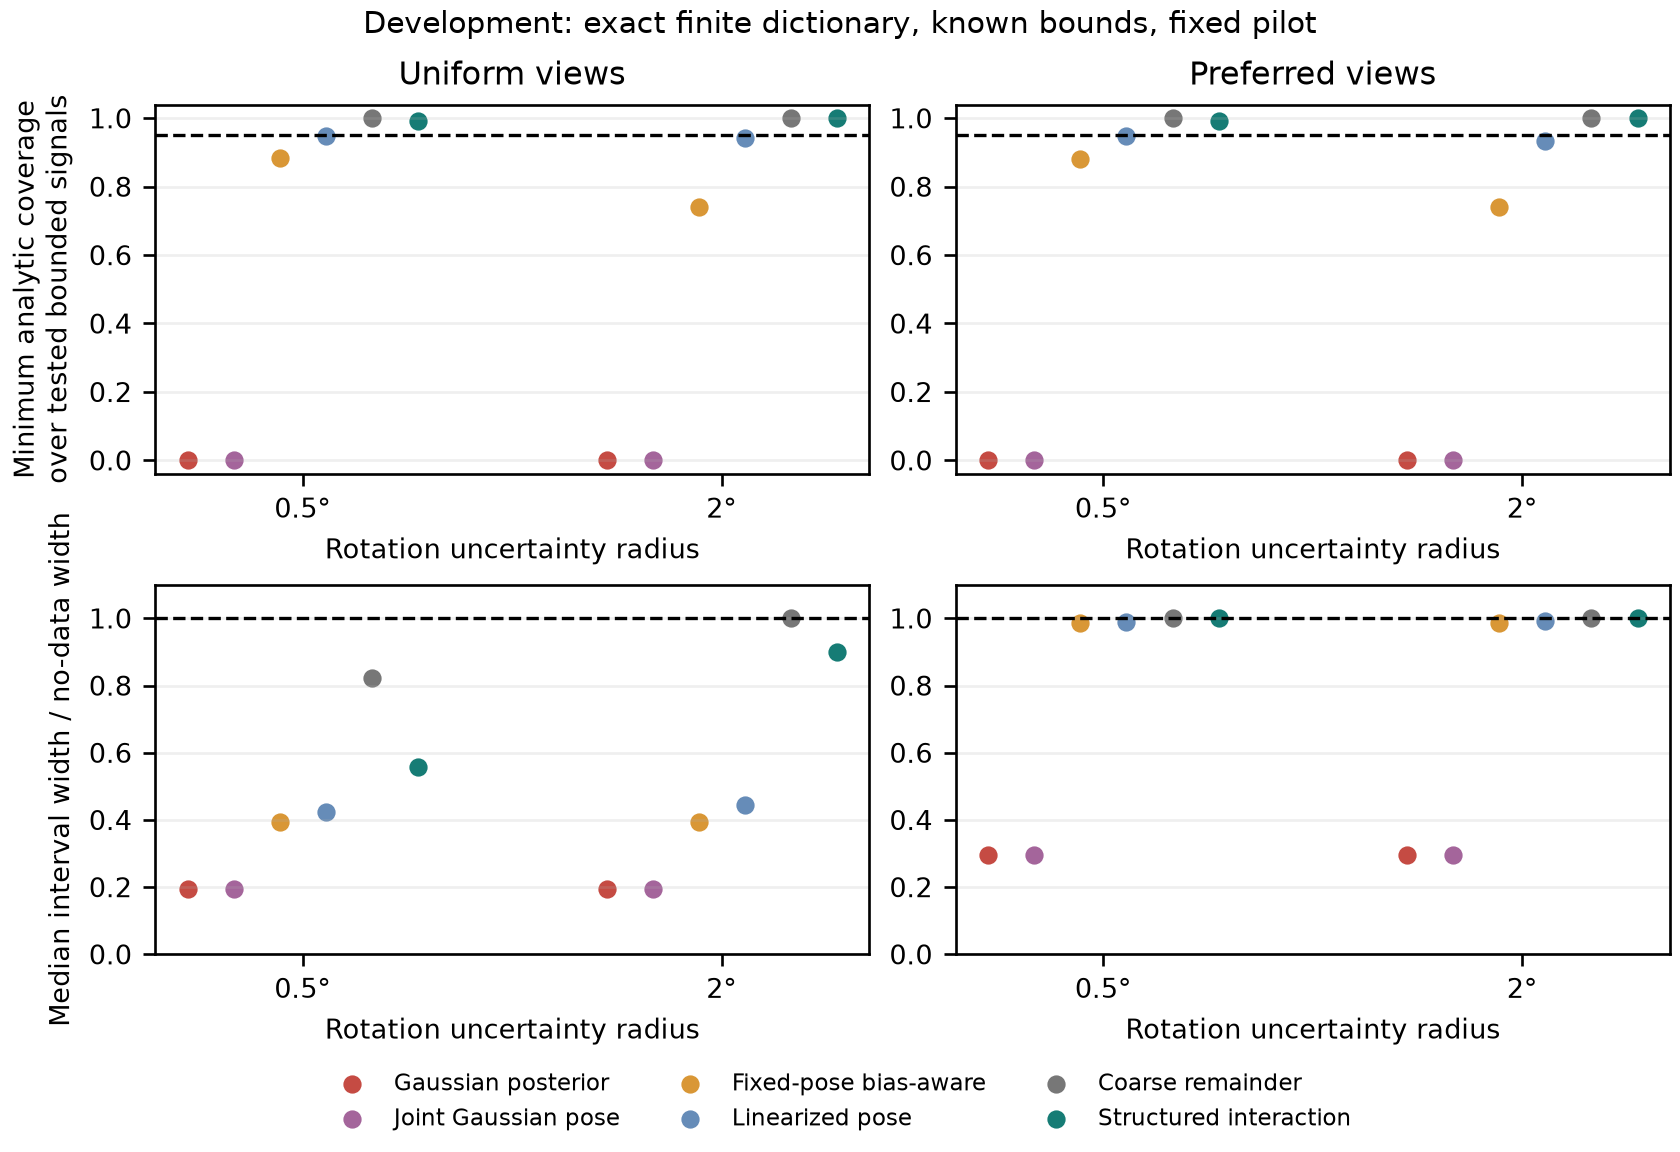
\includegraphics[width=.92\textwidth]{../results/uncertainty/development/coverage-summary/coverage-width.png}
\caption{Exact-dictionary development tests with known bounds and an independent fixed pilot. Minimum coverage is over the finite tested set, including adversarial signals; it is not an empirical proof of the worst case. Widths count each independent design once. Gaussian posterior methods separately pass their correctly matched prior-predictive coverage check at 0.95. Their fixed-parameter boundary failures do not contradict Bayesian prior-average calibration.}
\label{fig:coverage}
\end{figure*}
The structured certificate's smallest tested coverage was 0.991 at nominal 0.95; omitting the quadratic remainder gave 0.932. Median width relative to the no-data bound was 0.557 for broad views at $0.5^\circ$, and approximately one for preferred views. This is a usefulness limitation, not a calibration success to conceal with pooled averages.

\subsection{Ambient-space audit}
The fixed-pose audit uses 128 real acquisition geometries per dataset, a $24^3$ voxel grid, a spherical support of radius 0.35 times the field, and prescribed signal-to-noise power ratio 0.1. A pilot derived from real particles and each reference generator are normalized to unit voxel Euclidean norm. We set $B=2$ before seeing coverage; the triangle inequality covers all such normalized generator/pilot pairs. This simulation convention does not estimate the density radius of experimental data.

The initial dictionary has 33 non-null Gaussian modes. Two targets, a central average and an axial contrast, use Gaussian averaging widths 0.03 and 0.07 times the field. Restricted intervals, the same weights with a full-grid audit, enriched weights, and the ambient matrix-free solution use identical estimands. The larger-grid model is deliberately able to express errors outside the initial dictionary.
\begin{table*}[t]
\centering
\caption{Fixed-pose ambient audit: median interval width relative to the no-data width across two density targets. All three methods after auditing use the same supported voxel class. The first column instead assumes the initial 33-dimensional dictionary is correct and is not an honest interval for that larger class. All entries are development results.}
\label{tab:ambient}
\begin{tabular}{llrrrr}
\toprule
Dataset & Averaging width / field & Dictionary only & Same weights, audited & Enriched & Full matrix-free \\
\midrule
10028 & 0.03 & 0.008 & 0.978 & 0.689 & 0.687 \\
10028 & 0.07 & 0.007 & 0.510 & 0.053 & 0.050 \\
10049 & 0.03 & 0.020 & 1.016 & 0.718 & 0.716 \\
10049 & 0.07 & 0.020 & 0.636 & 0.075 & 0.073 \\
10076 & 0.03 & 0.024 & 0.949 & 0.721 & 0.719 \\
10076 & 0.07 & 0.023 & 0.462 & 0.072 & 0.072 \\
\bottomrule
\end{tabular}
\end{table*}

Table~\ref{tab:ambient} reports median widths across the two targets. The full-space solver reached its 0.5\% objective-gap tolerance in 12 of 12 cases, taking 2.4--11.1 seconds per target on the Mac. The enrichment solver reached the same outer tolerance in 8 of 12 cases within 100 rounds; nonconverged results retain valid bounds but do not establish optimality. The solvers optimize the conservative sum-width, so their sharper reported widths need not be ordered exactly by their objective gaps.

Dictionary-only intervals can be narrow because they exclude admissible density errors. For the EMPIAR-10028 central broad average, analytic coverage on the original, unregistered voxel-map generator is approximately $4.2\times10^{-5}$. The same image weights, with the ambient bias bound, cover at the prescribed level over the ambient ball. On each estimator's constructed ambient bias boundary, the audited intervals attain nominal 0.95 Gaussian coverage up to numerical tolerance. These boundary calculations check the theorem and implementation; they are not independent evidence of practical class calibration. Broader targets have substantially smaller relative widths than fine targets. The prescribed norm radius and fixed-pose assumption are essential to interpreting that result.


\subsection{Joint ambient and nonlinear pose uncertainty}
We combine the full supported voxel space with the nonlinear pose bound, using the broad axial contrast, 128 particles per geometry and the same prescribed density radius. Rotation radii are $0.1^\circ$, $0.5^\circ$ and $2^\circ$, with a shift radius of 0.01 working pixels in their joint unit ball. Signal cases include random density/pose boundaries, estimator-directed adversaries and the independent voxel reference under a coherent rotation. Table~\ref{tab:ambientpose} shows that a valid but conservative interval can still be uninformative at a large nuisance radius. Fixed-pose intervals reach coverage as low as 0.904 on these allowed perturbed cases. The nonlinear certificate's smallest tested analytic coverage is 0.9997; its conservatism requires scrutiny rather than being interpreted as superior calibration.
\begin{table}[t]
\centering
\caption{Joint ambient/pose interval width divided by the no-data width. Columns 2--4 use a 100-iteration cap. The last column repeats $2^\circ$ with up to 500 iterations; EMPIAR-10049 retains a 0.548\% gap, above the 0.5\% tolerance. Others meet tolerance. These are different optimization budgets, not separate independent replications.}
\label{tab:ambientpose}
\begin{tabular}{lrrrr}
\toprule
EMPIAR & $0.1^\circ$ & $0.5^\circ$ & $2^\circ$ & $2^\circ$, longer \\
\midrule
10028 & 0.087 & 0.200 & 0.866 & 0.865 \\
10049 & 0.118 & 0.239 & 0.996 & 0.992 \\
10076 & 0.110 & 0.218 & 0.910 & 0.907 \\
\bottomrule
\end{tabular}
\end{table}


We also compute the probability that the entire interval has the correct sign. For a positive true target and expected center $m$, this is $\Phi((m-q)/s)$, with the analogous negative-sign formula. The deposited-map axial contrasts are too small for the present bounds, despite high coverage. Central averages are easier (Table~\ref{tab:power}). The averaging standard deviation is 0.07 times the field, or approximately 16.5--33.8\,\AA; these coarse features do not establish ligand- or atomic-scale utility. Artificial perturbations directed along the target can be detected more readily, but are not substitutes for the deposited-map cases.
\begin{table}[t]
\centering
\caption{Probability that the nonlinear interval establishes the correct sign under the independent deposited-map generator and a coherent allowed rotation. Targets are broad averages or contrasts; these are not atomic-resolution claims. High coverage alone does not ensure detection.}
\label{tab:power}
\begin{tabular}{lrrrr}
\toprule
 & \multicolumn{2}{c}{Axial contrast} & \multicolumn{2}{c}{Central average} \\
EMPIAR & $0.1^\circ$ & $0.5^\circ$ & $0.1^\circ$ & $0.5^\circ$ \\
\midrule
10028 & 0.000 & 0.000 & 1.000 & 0.999 \\
10049 & 0.001 & 0.000 & 1.000 & 0.219 \\
10076 & 0.000 & 0.000 & 1.000 & 0.894 \\
\bottomrule
\end{tabular}
\end{table}


\subsection{Experimental reconstruction controls}
We execute stock cryoDRGN 4.3.1 homogeneous neural training on both exposure-group halves of all three stacks: three hidden layers, width 256, batch size eight, fixed consensus poses and CTFs. These are actual neural fits; they are not ab initio inference or uncertainty estimates. Gaussian and voxel ridge fits use the same halves. All methods are evaluated on identical held-out particles and 1,410 Fourier pairs per image inside radius 30 of the 64-pixel grid, with the same window and image-background normalization. Neural training itself uses the stock radius-32 loss and per-half global scaling, so training objectives are not identical.

Table~\ref{tab:reconstruction} records the completed 20-epoch checkpoint comparison. Continued improvement on tuning groups motivates longer neural runs. Exposure-group bootstrap comparisons, checkpoint hashes and direct-network versus map-Fourier checks are recorded with the results. FSC assesses conditional map agreement; neither it nor image prediction labels true experimental density coverage.
\begin{table}[t]
\centering
\caption{Experimental-image prediction error on development test groups (normalized MSE; lower is better). Neural runs are 20-epoch checkpoints; convergence is still being assessed. All half-map FSCs remain above 0.143 through the sampled limit in the last column, which is not a measured crossing.}
\label{tab:reconstruction}
\begin{tabular}{lrrrr}
\toprule
EMPIAR & Gaussian & Voxel & Neural & Limit (\AA) \\
\midrule
10028 & 0.8355 & 0.8417 & 0.8330 & 16.08 \\
10049 & 0.9308 & 0.9316 & 0.9309 & 7.87 \\
10076 & 0.8764 & 0.8806 & 0.8740 & 13.97 \\
\bottomrule
\end{tabular}
\end{table}


\subsection{Baselines and numerical checks}
Implemented matched mathematical baselines include full Gaussian posterior covariance, diagonal variational covariance, regularized sampling covariance, joint Gaussian pose covariance, identifiable unregularized estimation, fixed-pose bias-aware intervals, coarse and structured nuisance bounds, and the no-data interval. These are not executions of every external paper's original code. Full Gaussian posteriors pass their exactly matched linear prior-predictive identity at 0.95. Narrow priors can nevertheless fail bounded fixed-signal tests; wider priors and unregularized estimation can produce very wide intervals.

Independent conic optimization checks the majorization, primal-dual and ambient solvers on small instances. Derivative finite differences, nonlinear remainder tests, direct Fourier sums, adjoint identities and independent Gaussian-integral checks validate implementation components. The current suite has 35 passing tests, including a three-dimensional Fourier-transform check for externally generated maps. Tight FINUFFT tolerances are numerical checks, not interval-arithmetic guarantees on roundoff.

\section{Limitations and Work Remaining}
The current evidence does not establish an end-to-end uncertainty method with estimated poses, noise law and density class. Local pose radii and the total density bound are assumptions. Selecting them from the same inference residuals would require new analysis; a narrow residual does not rule out an almost invisible density error. Learned support can exclude true structure. Gauge and hand ambiguity must be fixed or included in the target class.

The next validation must freeze the method before fresh simulations and additional source groups, include higher bandwidth and grid refinement, complete bootstrap and neural convergence comparisons, and test correlated noise, CTF errors, heterogeneity and support violations. The power analysis above is only an initial coarse-feature check. Simultaneous maps need multiplicity correction. Real-data prediction and stability cannot supply unavailable density-coverage labels. Comprehensive literature screening and independent review of a complete candidate remain outstanding.

\section*{Reproducibility and Impact}
The active research branch is \texttt{uncertainty-study} at \url{https://github.com/yashpatel5400/fourier-cryo-splats}. It preserves failed development approaches and distinguishes them from completed outputs. The earlier reconstruction release v0.1.0 remains available with its conditional FSC results; it is not the uncertainty study's accuracy claim. No new conference submission or acceptance is implied by this format. Background PDFs are retained locally with source hashes rather than redistributed. Prematurely calibrated-looking maps can mislead structural interpretation; explicit assumptions and negative controls are central outputs of this work.

\bibliography{references,uncertainty-references}
\bibliographystyle{icml2026}
\clearpage
\appendix
\section{Additional Derivations}
\subsection{An identifiability lower bound}
\begin{proposition}
Let two allowed parameters induce $N(\mu_0,I)$ and $N(\mu_1,I)$, with targets $t_0,t_1$. Any interval covering each target with probability at least $1-\alpha$ has expected length under the first law at least
\begin{equation}
|t_1-t_0|[1-2\alpha-\operatorname{TV}(P_0,P_1)]_+,
\end{equation}
where $\operatorname{TV}(P_0,P_1)=2\Phi(\norm{\mu_1-\mu_0}/2)-1$.
\end{proposition}
\begin{proof}
Under $P_0$, the probability of containing $t_1$ is at least $1-\alpha-\operatorname{TV}(P_0,P_1)$ by the definition of total variation. The union bound gives simultaneous containment of both targets with probability at least the displayed positive part. The length on that event is at least their separation. The total variation formula follows by projecting onto the line between the Gaussian means.
\end{proof}
This standard two-point argument also applies to different allowed nuisance settings. Exact null directions give a nonvanishing uncertainty floor even with perfect image prediction. It does not assert that a finite numerical search finds the largest possible separation.

\subsection{Gaussian density-energy Gram matrix}
For isotropic paired features, let
\begin{align}
P_{jk}&=\left(\frac{2\pi\sigma_j^2\sigma_k^2}{\sigma_j^2+\sigma_k^2}\right)^{3/2}
\exp\left[-\frac{\norm{\mu_j-\mu_k}^2}{2(\sigma_j^2+\sigma_k^2)}\right],\\
Q_{jk}&=P_{jk}\text{ with }\mu_j-\mu_k\text{ replaced by }\mu_j+\mu_k.\nonumber
\end{align}
Integrating products of Gaussians and applying Parseval gives real and imaginary coefficient blocks $2(P+Q)$ and $2(P-Q)$, with zero cross block. A zero-centered imaginary coefficient is exactly null. Numerically excluded eigenmodes are reported; exclusion changes the stated Gaussian subspace. In an ambient audit they remain available to the larger space rather than being silently assigned zero uncertainty.

\subsection{Uniform nonlinear remainder}
For a Gaussian of width $\sigma$ at radial distance $r$, bounds on value, gradient and Hessian are
\begin{align}
g_0(r)&=e^{-r^2/(2\sigma^2)},\\
g_1(r)&=r g_0(r)/\sigma^2,\\
g_2(r)&=(1+r^2/\sigma^2)g_0(r)/\sigma^2.
\end{align}
On an interval of possible distances, $g_0$ is largest at the lower endpoint; $g_1$ and $g_2$ attain their largest value at the point nearest $\sigma$. A rotation radius $a\le\pi$ gives displacement at most $2\norm{k}\sin(a/2)$, speed at most $a\norm{k}$ and acceleration at most $a^2\norm{k}$. A shift radius $s$ gives phase speed at most $2\pi\norm{q}s/\text{box}$.

The product rule bounds the second derivative by the sum of squared-speed times $g_2$, acceleration times $g_1$, twice speed times phase-speed times $g_1$, and squared phase-speed times $g_0$. Sum conjugate-pair bounds and apply the fixed CTF/noise scale. A coefficient-column Frobenius bound controls the operator term; the pilot-weighted bound controls its pilot term. Taylor's integral formula gives Equation~\eqref{eq:pose}. Evaluating a Hessian only at the nominal pose would not establish this uniform result.

\subsection{Retaining quadratic pose terms}
The isotropic quadratic remainder can dominate an interval. A development extension retains the curvature and uses a cubic remainder instead. Put $E_{iab}=\partial^2 A_i/\partial u_{ia}\partial u_{ib}$ at zero, $Q_i(w)_{ab}=w_i^\top E_{iab}\rho_0$, and let $U_i(w)$ collect columns $E_{iab}^\top w_i$ over all ordered pairs. Since $\norm{u_i\otimes u_i}_F\le1$, a valid bias bound is
\begin{align}
b_2(w)&=B\norm{\ell-\A^*w}+\sum_i\norm{J_i^\top w_i}\nonumber\\
&\quad+B\sum_i\norm{T_i(w)}_F+\tfrac12\sum_i\norm{Q_i(w)}_F\nonumber\\
&\quad+\tfrac B2\sum_i\norm{U_i(w)}_F+\sum_i\gamma_{3i}\norm{w_i}.
\end{align}
For a Fourier voxel column, define $T(q,x)=2\pi a^3\norm{k}\norm{x}/d$. Its third derivative along any allowed pose segment is bounded by $|C|[L^3+3LH+T]$ before whitening. The three summands follow by differentiating the phase exponential three times. Pilot contraction and a column Frobenius bound give $H_{3i}$ and $K_{3i}$, hence $\gamma_{3i}=(H_{3i}+BK_{3i})/6$. Taylor's integral remainder and Cauchy--Schwarz then give Theorem~\ref{thm:coverage} with $b_2$. Sharing of density errors and rank-one quadratic pose constraints are still relaxed.

Analytic column Hessians and pixel-space Gram factors implement these Euclidean groups. Mixed finite differences and independent nonlinear projections test the implementation. The initial EMPIAR-10028 contrast probe reduces width/no-data from 0.200 to 0.143 at $0.5^\circ$ and from 0.865 to 0.478 at $2^\circ$. Broader comparisons are running; a single favorable probe is not the final evaluation.

\subsection{An independent noise-scale upper bound}
Known noise is not necessary if an independently calibrated upper bound is available. A standard construction assumes independent calibration coordinates $z_j=\mu_j+\sigma e_j$, $e_j\sim N(0,1)$, with arbitrary fixed means and independent inference noise. For $\nu$ coordinates, set
\begin{equation}
\overline\sigma=\norm{z}/\sqrt{\chi^2_{\nu,\beta}}.
\end{equation}
The probability that $\overline\sigma\ge\sigma$ is at least $1-\beta$: the central chi-square pivot is exact at zero mean, and a noncentral chi-square has a smaller lower tail. Conditional on calibration, weights may use $\overline\sigma$. On this event their inference standard deviation is at most $s_+=\overline\sigma\norm{w}$. For $\alpha<1/2$, $q(s_+,b,\alpha)\ge b$, and Gaussian coverage decreases with the actual noise standard deviation up to $s_+$. Integrating the conditional bound yields coverage at least $(1-\alpha)(1-\beta)\ge1-\alpha-\beta$.

This extension does not justify independence of windowed Fourier pixels or estimate arbitrary covariance. With 128 calibration coordinates and $\beta=0.01$, a 20,000-draw development control gives scale-bound failure 0.0103 under independence. Equicorrelation 0.5 raises that failure to 0.503. Such a calibration set violates the premise even if a particular resulting interval remains conservative. Experimental whitening remains unresolved.

\subsection{Simultaneous targets and sensitivity budgets}
For $K$ targets and parameter-budget choices fixed independently of inference noise, applying Theorem~\ref{thm:coverage} with $\alpha/K$ gives simultaneous coverage by the union bound. Correlated Gaussian maxima can reduce the noise component if the joint weight covariance is accounted for. Selecting the most favorable point on a sensitivity surface after inspecting inference data requires such simultaneous control. A density radius supplied by simulation truth is an oracle control and cannot be reported as a practical calibration method.

\section{Survey and Experimental Audit Trail}
The repository's living survey distinguishes density uncertainty, pose uncertainty, conformational variability/populations, map-processing confidence and atomic-model uncertainty. Its broad Europe PMC retrieval ledger contains 16,969 deduplicated records, mostly application papers; that count is not a count of reviewed methods. The curated list contains 86 candidate works at this draft checkpoint, with local full-text availability recorded separately. Recent items include LocScale-2.0, CryoDiff, CryoSplat, GEM, measurement-limited heterogeneity, population-counting work and the CAHRA dataset-construction preprint. Preprints and final publications are distinguished, and titles/versions are checked against primary sources.

The full experimental protocol draft records unimplemented comparisons and required failure controls. Fixed-pose resampling must be distinguished from rerunning alignment; a mathematical diagonal-Gaussian control must be distinguished from reproducing Ullrich et al.'s full software; cryoDRGN backprojection must be distinguished from training a neural model. Exposure-group splits do not undo the dependence introduced by full-data consensus poses. All development results, including the initially incomplete covariance-factor benchmark, remain identifiable by filename and status.
\end{document}
